\clearpage
\myparagraph{\olly}
\myindex{\olly}

Загрузим этот пример в \olly. 
Входное значение для функции пусть будет \TT{0x12345678}.

Для $i=1$, мы видим, как $i$ загружается в \ECX: 

\begin{figure}[H]
\centering
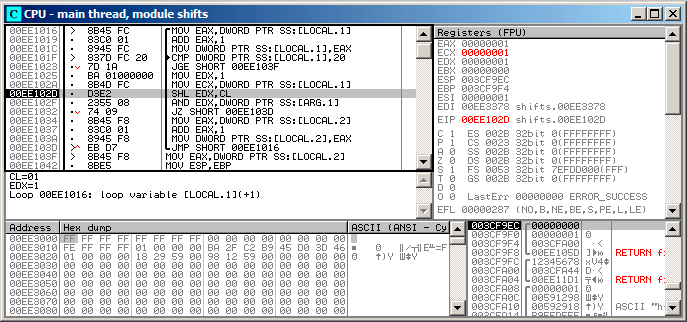
\includegraphics[scale=\FigScale]{patterns/14_bitfields/4_popcnt/olly1_1.png}
\caption{\olly: $i=1$, $i$ загружено в \ECX}
\label{fig:shifts_olly1_1}
\end{figure}

\EDX содержит 1. Сейчас будет исполнена \SHL.

\clearpage
\SHL исполнилась:

\begin{figure}[H]
\centering
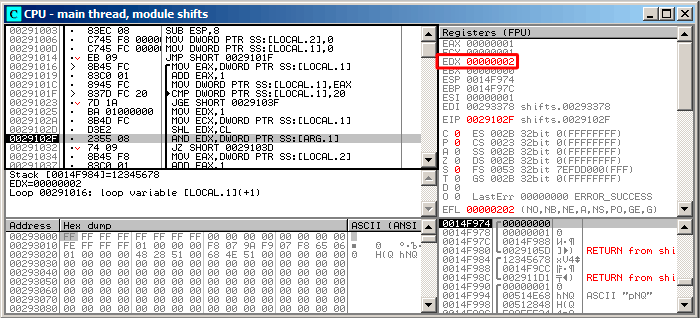
\includegraphics[scale=\FigScale]{patterns/14_bitfields/4_popcnt/olly1_2.png}
\caption{\olly: $i=1$, \EDX=$1 \ll 1=2$}
\label{fig:shifts_olly1_2}
\end{figure}

\EDX содержит $1 \ll 1$ (или 2). Это битовая маска.

\clearpage
\AND устанавливает \ZF в 1, 
что означает, что входное значение (\TT{0x12345678}) 
умножается\footnote{Логическое \q{И}} с 2 давая в результате 0:

\begin{figure}[H]
\centering
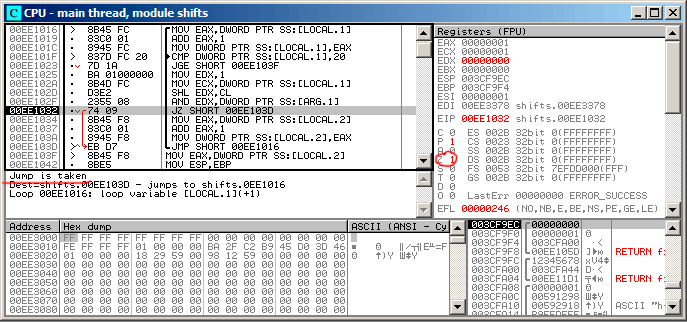
\includegraphics[scale=\FigScale]{patterns/14_bitfields/4_popcnt/olly1_3.png}
\caption{\olly: $i=1$, есть ли этот бит во входном значении? Нет.
 (\ZF=1)}
\label{fig:shifts_olly1_3}
\end{figure}

Так что во входном значении соответствующего бита нет.
Участок кода, увеличивающий счетчик бит на единицу, не будет исполнен: инструкция \JZ \emph{обойдет} его.

\clearpage
Немного потрассируем далее и $i$ теперь 4.%

\SHL исполнилась:

\begin{figure}[H]
\centering
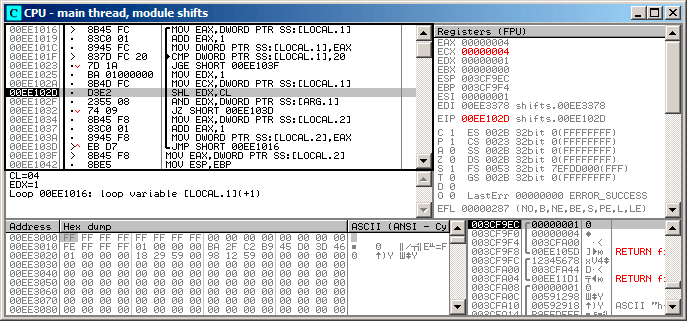
\includegraphics[scale=\FigScale]{patterns/14_bitfields/4_popcnt/olly4_1.png}
\caption{\olly: $i=4$, $i$ загружено в \ECX}
\label{fig:shifts_olly4_1}
\end{figure}

\clearpage
\EDX=$1 \ll 4$ (или \TT{0x10} или 16): 

\begin{figure}[H]
\centering
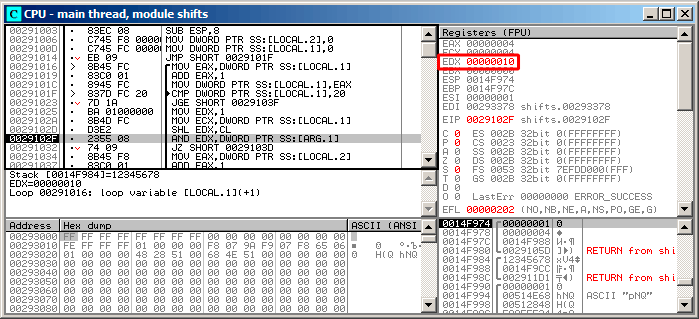
\includegraphics[scale=\FigScale]{patterns/14_bitfields/4_popcnt/olly4_2.png}
\caption{\olly: $i=4$, \EDX=$1 \ll 4=0x10$}
\label{fig:shifts_olly4_2}
\end{figure}

Это ещё одна битовая маска.

\clearpage
\AND исполнилась:

\begin{figure}[H]
\centering
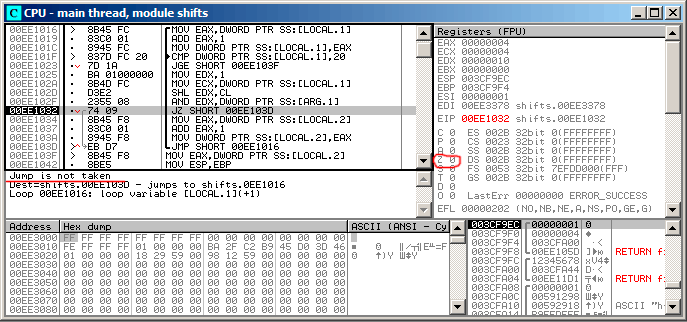
\includegraphics[scale=\FigScale]{patterns/14_bitfields/4_popcnt/olly4_3.png}
\caption{\olly: $i=4$, есть ли этот бит во входном значении? Да.  (\ZF=0)}
\label{fig:shifts_olly4_3}
\end{figure}

\ZF сейчас 0 потому что этот бит присутствует во входном значении.
Действительно, \TT{0x12345678 \& 0x10 = 0x10}. 
Этот бит считается: переход не сработает и счетчик бит будет увеличен на единицу.

Функция возвращает 13. 
Это количество установленных бит в значении \TT{0x12345678}.
